\documentclass[10pt,a4paper]{article}
\usepackage[T1]{fontenc}
\usepackage[utf8]{inputenc}
\usepackage[spanish,es-tabla]{babel}
\parindent=0cm %Modificar tamaño de sangria
\usepackage{amsmath}
\usepackage{amssymb,amsfonts,latexsym,cancel}
\usepackage{graphicx}
\usepackage{epstopdf}
\usepackage{float}
\usepackage{subfigure}
\usepackage{array}
\usepackage{longtable}
\newcolumntype{E}{>{$}c<{$}}
\setcounter{MaxMatrixCols}{40}
\usepackage{bm}
\usepackage{xcolor}
%%%%%%%%%%%%%%%%%%%%%%%%%%%%%%%%%%%%%
%%%PAQUETES O CONFIGURACION NUEVA%%%%
%%%%%%%%%%%%%%%%%%%%%%%%%%%%%%%%%%%%%
\usepackage[lmargin=2cm, rmargin=2cm,top=2.5cm,bottom=2cm]{geometry}
\usepackage{fancyhdr}
\pagestyle{fancy}
\fancyhead{}%%Es para limpiar el documento
\fancyhead[C]{Metaheurística}
\fancyhead[R]{
\includegraphics[scale=0.07]{figuras/logo}}
\fancyfoot{}
\fancyfoot[R]{\thepage}
\fancyfoot[L]{Bryan Ricardo}
\renewcommand{\headrulewidth}{0.9pt}
\renewcommand{\footrulewidth}{0.5pt}
\usepackage{xcolor}
\providecommand{\abs}[1]{\lvert#1\rvert}
\providecommand{\norm}[1]{\lVert#1\rVert}
\usepackage{ mathrsfs }
%%%%%%%%%%%%%%%%%%%%%%%%%%%%%%%%%%%%%
%%INTEGRALES INFERIORES Y SUPERIORES
\usepackage{amsmath}
\def\upint{\mathchoice%
    {\mkern13mu\overline{\vphantom{\intop}\mkern7mu}\mkern-20mu}%
    {\mkern7mu\overline{\vphantom{\intop}\mkern7mu}\mkern-14mu}%
    {\mkern7mu\overline{\vphantom{\intop}\mkern7mu}\mkern-14mu}%
    {\mkern7mu\overline{\vphantom{\intop}\mkern7mu}\mkern-14mu}%
  \int}
\def\lowint{\mkern3mu\underline{\vphantom{\intop}\mkern7mu}\mkern-10mu\int}
%%%%%%%%%%%%%%%%%%%%%%%%%%%%%%%%%%%%%%%%%%%%%%%
\begin{document}
\begin{titlepage}
\begin{center}
\vspace*{2\baselineskip}%%saltos de linea
\hrule height 3pt
\vspace*{0.5\baselineskip}%%saltos de linea
{\Huge \textbf{Universidad Autonoma de Aguascalientes}}
{\Large \textbf{LICENCIATURA EN MATEMATICAS APLICADAS}}
\vspace*{0.5\baselineskip}%%saltos de linea
\hrule
\vspace*{0.5\baselineskip}%%saltos de linea

\includegraphics[scale=0.5]{figuras/logo}
\vspace*{2\baselineskip} \\%%saltos de linea
\textbf{\large MATERIA: Metaheurística} \\
\vspace*{1.5\baselineskip}
\textbf{\large DOCENTE: EUNICE ESTHER PONCE DE LEON SENTI } \\
\vspace*{1.5\baselineskip}
\textbf{\large FECHA DE CREACION: 13 de agosto de 2023} \\  
\vspace*{3\baselineskip}
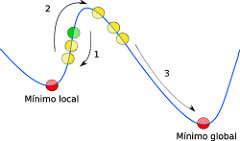
\includegraphics[scale=1.2]{figuras/imagen}
\vfill
BRYAN RICARDO BARBOSA OLVERA \\
\today \\

\end{center}
\end{titlepage}


\LARGE
\section{Criterio de la primera derivada}

1-Dar un funcion $f$ continua en $ \left[ a,b \right] $ \\
2-Encontrar un punto critico $c$ en $ \left( a,b \right)  $ \\
3-Si $ f^{\prime} \left( x \right) \geq 0   $ para $x \ \in \ \left( a,c \right)  $ y $ f ^{\prime} \left( x \right) \leq 0  $
para $ x \ \in \ \left( c,b \right)  $ entonces $f$ tiene un máximo relativo en $c$. \\
4-Si $ f^{\prime} \left( x \right) \leq 0   $ para $x \ \in \ \left( a,c \right)  $ y $ f ^{\prime} \left( x \right) \geq 0  $
para $ x \ \in \ \left( c,b \right)  $ entonces $f$ tiene un mínimo relativo en $c$. \\
5-Si $f^ {\prime} \left( x \right) > 0 $ para $x \ \in \left( a,c \right)  $ y $ f^{\prime} \left( x \right) >0   $ para 
$x \ \in \ \left( c,b \right)  $ o $ f^{\prime} \left( x \right) <0  $ para $x \ \in \ \left( a,c \right)  $ y 
$ f^{\prime} \left( x \right) <0 $ para $ x \ \in \ \left( c,b \right)  $, entonces $f$ no tiene ni un máximo ni un mínimo 
relativo en $c$.

\section{Criterio de la segunda derivada}
1-Dar una funcion $f$ diferenciable en una vecindad $ \left( a,b \right)  $. \\
2-Sea $c \ \in \ \left( a,b \right) \ \wedge \ f^{\prime} \left( c \right) =0 $.  \\
3-Verificamos que $f^{\prime \prime} \left( c \right) $ exista.\\
4-Si $f^{\prime \prime} \left( c \right)  < 0$, entonces $f$ tiene un máximo relativo en $c$.\\
5-Si $f^{\prime \prime} \left( c \right)   > 0$, entonces $f$ tiene un minimo relativo en $c$.\\

\section{Criterio de maximos y minimos en funciones reales de variable vectorial}
1-Dar una funcion $f: \mathbb{R}^2 \rightarrow \mathbb{R} $ que pertenesca a la clase $C^2$ en una vecindad 
$ \mathscr{S} \left( x_0 ; r \right) $ de $x_0$. \\
2-Verificar que $D_1 f \left( x_0 \right) = D_2 f \left( x_0 \right) =0. $\\ 
3-Si $D_{11} f \left( x_0 \right) D_{22} f \left( x_0 \right) - \left( D_{12} f \left( x_0 \right)  \right)^2 >0 $ 
entonces $f$ tiene un valor extremo en $x_0$. \\
3.1-Si $D_{11} f \left( x_0 \right)<0  $ tiene un máximo relativo.  \\
3.2-Si $D_{11} f \left( x_0 \right)>0  $ tiene un mínimo relativo.  \\
4.Si $D_{11} f \left( x_0 \right) D_{2 2} f \left( x_0 \right) - \left( D_{12} f \left( x_0 \right)  \right) ^2 <0 $. 
entonces $f$ no tiene un valor extremo en $x_0$; tiene un punto silla.

\end{document}
